%
%
%
\chapter{The Static Conductivity in the Spin Fermion Model including Umklapp Scattering}
\label{ch:calculation}
%
%
%
The static electrical conductivity $\sigma_{\mt{dc}}$ is computed in this chapter, using the memory-matrix-formalsim.
The underlying model is the spin-fermion-model (see chapter \ref{ch:spin fermion model}), including umklapp scattering that breaks translation symmetry.
In this chapter, our focus lies on the physical analysis of the obtained expression for the conductivity.
An explicite computation is demonstrated in appendix \ref{appch:static susceptibility} and \ref{appch:green function}.

%
%
%\section{Static Conductivity's Derivation}
%\label{sec:deviation conductivity}
%
%
Two physical objects, fermions near the Fermi surface and spin fluctuations, are considered in the spin-fermion-model as introduced in the previous chapter.
Spin fluctuations are generated at the vicinity of an antiferromagnetic quantum critical point due to particle-holes-excitations.
Fermions, located at the point $\vb{k}$ and $\vb{k}+\vb{Q}$ on the Fermi suface, are connected to each other because of these fluctuations.
The momentum conservation of the spin-fermion-model Hamiltonian has been shown in the previous chapter.
The static electrical conductivity is thus infinite as it is poven in chapter \ref{ch:infinite conductivity}.
Considering umklapp scattering, the translation symmetry is broken and the momentum is unconserved.
As a conseuqence the static conductivity becomes finite.
This calculation is presented here.

The memory-matrix-formalism is used in chapter \ref{ch:memory matrix formalism} to derivate the following formula for the static electrical conductivity, including the spin-fermion-model as well as umklapp scattering.
%
\begin{align}
	\sigma_{\mt{dc}} = -\lim\limits_{z \to 0} \frac{z \cdot |\chi_{\mt{JP}}(\omega = 0)|^{2}}{\mathcal{G}_{\dot{\mt{P}}\dot{\mt{P}}}(\vb{k}, z)}
	\label{eq:static conductivity formula}
\end{align}
%
Here, $z$ is a complex frequency and $\chi_{\mt{JP}}(\omega = 0)$ is the static susceptibility between current and momentum.
The Green function in the denominator is given by
%
\begin{align}
	\mathcal{G}_{\dot{\mt{P}}\dot{\mt{P}}}(\vb{k}, z) = \int\limits_{0}^{\infty} \dd{t} e^{izt} \expval{\comm{\dot{\mt{P}}(t)}{\dot{\mt{P}}(0)}_{-}}_{0},
	\label{eq:Green function}
\end{align}
%
where the usual quantum mechanical commutator is used, indicated with the minus sign at the squared brackets.
The expectation value is evaluated with respect to the unpertubative Hamiltonian H, visualized with the index 0.
The interaction between fermions and spin fluctuations is included in the Hamiltonina H.
The time derivative of momentum is given by equation \eqref{eq:time derivative momentum finite}.

The possible temperature dependence of the Green function $\mathcal{G}_{\dot{\mt{P}}\dot{\mt{P}}}(\vb{k}, z)$ and the static susceptibiliy $\chi_{\mt{JP}}(\omega = 0)$ is investigated.
The latter is expected to be temperature independent, since both quantities are not explicitly time dependent. \todo{right or wrong?}
This calculation is shown in detail in the appendix \ref{appch:static susceptibility}, using the diagrammatic pertubation technique.
The considered diagrams are the electron-pair bubble for each species of fermions, depicted in figure \ref{fig:static susceptibility}.
Therefore, the obtained expression of the susceptibility is given by
%
\begin{align}
	\chi_{\mt{PJ}}(\omega = 0) = \frac{\sqrt{m_{1} m_{2}}}{\pi} T \cdot \ln(e^{\flatfrac{\mu}{T}} + 1),
	\label{eq:static susceptibility computed}
\end{align}
%
where the chemical potential is denoted as $\mu$.
The logarithm is approximated in the limit of small temperatures ($\mu \gg T$) to $\ln(e^{\flatfrac{\mu}{T}} + 1) \rightarrow \flatfrac{\mu}{T}$.
The temperature cancels when this expression is inserted and the static susceptibility is given by constant parameters, $\chi_{\mt{PJ}}(\omega = 0) = \flatfrac{\mu\sqrt{m_{1} m_{2}}}{\pi}$.
The chemical potential is assumed to be temperature independent in the observed regime.

%
\begin{figure}
	\centering
	\includegraphics[width=0.4\textwidth]{spin_wave_bubble.eps}
	\caption{
The zeroth order bubble diagram is shown for spin density fluctuations.
The wavy lines symbolizes the spin density wave, denoted as $\mathcal{D}_{\mu}(\vb{k},i\omega_{n})$.
The momentum of lower line is modified by the vector $\vb{G}$, originated from umklapp scattering.
	}
	\label{fig:spin wave bubble}
\end{figure}
%
The only temperature dependence of the static electrical conductivity emerges hence by the Green function $\mathcal{G}_{\dot{\mt{P}}\dot{\mt{P}}}(\vb{k}, z)$.
Only the free bubble diagram is considered when calculating the Green function with diagrammatic pertubation theory, which is depicted in figur \ref{fig:spin wave bubble}.
Higher order terms in the diagrammatic treatment are corrections of the bubble diagram.
Therefore the conductivity or resistance is only determined by spin fluctuations.
Resistance is a consequence of fermionic coupling to other degrees of freedom, obtained as finite fermionic lifetime.
It is thus proportional to the imaginary part of the retarded Green function $\mathcal{G}_{\dot{\mt{P}}\dot{\mt{P}}}^{\mt{ret}}(\vb{k}, z)$.
Appendix \ref{appch:green function} shows the detailed computation of the expression of the retarded Green function.
%
\begin{align}
	\Im{\mathcal{G}_{\dot{\mt{P}}\dot{\mt{P}}}^{\mt{ret}}(\vb{k}, \omega)} &= 
		-\frac{4 \gamma^{2} \beta \omega}{\pi}
		\sum\limits_{\vb{Q}_{1}, \vb{Q}_{2}}
		\sum\limits_{\vb{G}}
		\vert \mt{J}_{\vb{G}} \vert^{2}
		\int\limits_{0}^{\infty} \dd{\epsilon}
		\frac{\epsilon^{2} e^{\beta \epsilon}}{(e^{\beta \epsilon} - 1)^{2}}
		\notag \\
		&\times
		\int_{\vb{k}} G_{j}^{2} \cdot
		\frac{1}{(\vb{k}+\vb{G}-\vb{Q}_{1})^{4} + \gamma^{2} \epsilon^{2}} \cdot
		\frac{1}{(\vb{k} + \vb{Q}_{2})^{4} + \gamma^{2} \epsilon^{2}}
\end{align}
%
The integral is extended over the first Brillouin zone.
The periodicity of the spin susceptibility and pertubation is considered by the sums over $\vb{Q}_{i}$ ($i=1,2$) and $\vb{G}$, respectivily.
In both cases these are reciprocal lattice vectors.
Spatial direction of the momentum is represented by the index $j$ and $\beta^{-1} = T$.
The obtained integrals are now investigated with respect to different cases since their are not exactly solvable.
%
%
%\section{Analysis of the static conductivity}
%\label{sec:analysis conductivity}
%
%

The intergal converges if the magnitude of one of the momentum terms, $\vb{k}+\vb{G}-\vb{Q}_{1}$ or $\vb{k} + \vb{Q}_{2}$, is large.
Since both terms are of the power of four, the integral is a fast decreasing function in the large momentum limit.
The integral diverges, if these terms are zero and this happens in many constellations.
One of the most divergent one is assumed in the following approach.
The vector $\vb{k}$ is limited to the first Brillouin zone and the reciprocal lattice vectors are set to $\vb{G} = \vb{Q}_{1}$ and $\vb{Q}_{2} = 0$.
The choice of the reciprocal lattice vectors is arbitrary and it is therefore possible that the $j$-component of $\vb{G}$ is large.
This divergence is killed by the coupling parameter $\mt{J}_{\vb{G}}$ that is assumed to be fast decreasing for large $|\vb{G}|$.

The remaining momentum integral is now exactly integrable.
First of all, the momentum and frequency variables are transformed into dimensionles variables, using the transformation rules $\vb{k} = \vb{y} \cdot \sqrt{\gamma T}$ and $\epsilon = x \cdot T$, respectivily.
The new variable $\vb{y}$ is further transformed into plane polar coordinates.
The upper limit of the radius $|\vb{y}|$ is set to infinity, since the integrand is decreasing fast to zero for $|\vb{y}| \to \infty$.
As a consequence the angular integral is easily evaluated, yielding the factor $2\pi$.
The remaining integral is given by the following expression.
%
\begin{align}
	\Im{\mathcal{G}_{\dot{\mt{P}}\dot{\mt{P}}}^{\mt{ret}}(\vb{k}, z)} = 
		 -\frac{2 \cdot G_{j}^{2} \cdot \vert \mt{J}_{\vb{K}} \vert^{2}}{\gamma \cdot \pi^{2}} \cdot \frac{\omega}{T}
		\int\limits_{0}^{\infty} \dd{x}
		\frac{x^{2} e^{x}}{(e^{x} - 1)^{2}}
		\int\limits_{0}^{\infty} \dd{y}
		\frac{y}{\big(y^{4} + x^{2}\big)^{2}}
\end{align}
%
The $y$-integral is substituted one last time, using the transformation rule $y^{2} = z \cdot x$.
The obtained integral is evaluated to $\flatfrac{\pi}{4}$, using the integral formula \eqref{eq:integral1}.
Both limits, $x \to 0$ and $x \to \infty$, of the intergal over $x$ are investigated.
In the case of large $x$, the integral is decreasing fast to zero due to the ratio of the exponential functions.
The upper limit is thus set to one and the integrand is expanded for small values of $x$.
In first order the integrand is approximated to $\flatfrac{1}{x^{3}}$.
This is a highly divergent function in the limit $x \to 0$ and as a consequence the static conductivity is divergent as well.

The result of a divergent conductivity is surely incorrect in a system with broken translation symmetry.
In chapter \ref{ch:infinite conductivity}, it is shown that translation symmetry and the consequent conserved momentum causes an infinite conductivity in the static limit.
Chapter \ref{ch:spin fermion model} shows, that momentum is conserved in the unpertubated spin-fermion-model \eqref{eq:time derivative momentum}, while it is unconserved considering umklapp scatering \ref{eq:time derivative momentum finite}.
As a concequence, a finite static conductivity is expected instead of divergence.

The origin of this discrepancy is supposed to be in the choice of the control parameter $r$.
The paramter $r$ is assumed to be zero, since its proportional to $\xi^{-2}$ and the correlation length $\xi$ diverges at the quantum critial point.
This assumption is incorrect in the sence that the system is not directly at the quantum cirtical point, but rather in the vicinity of him.
The system is supposed to be in the quantum critical phase, see figure \ref{fig:phase diagram}, at a point with tuning parameter $\mt{g} = \mt{g}_{\mt{c}}$ and temperature $ T > 0$.
While the temperature is decreased to get closer to the quantum critical point, the tuning parameter is fixed.
Considering a finite value of the control parameter $r$, the imaginary part of the retareded Green function is given by
%
\begin{align}
	\Im{\mathcal{G}_{\dot{\mt{P}}\dot{\mt{P}}}^{\mt{ret}}(\vb{k}, z)} &= 
		-\frac{4 \gamma^{2} \beta \omega}{\pi}
		\sum\limits_{\vb{Q}_{1}, \vb{Q}_{2}}
		\sum\limits_{\vb{G}}
		\vert \mt{J}_{\vb{G}} \vert^{2}
		\int\limits_{0}^{\infty} \dd{\epsilon}
		\frac{\epsilon^{2} e^{\beta \epsilon}}{(e^{\beta \epsilon} - 1)^{2}}
		\notag \\
		&\times
		\int_{\vb{k}} G_{j}^{2} \cdot
		\frac{1}{((\vb{k}+\vb{G}-\vb{Q}_{1})^{2} + r)^{2} + \gamma^{2} \epsilon^{2}} \cdot
		\frac{1}{((\vb{k} + \vb{Q}_{2})^{2} + r)^{2} + \gamma^{2} \epsilon^{2}}
\end{align}
%
The approach to solve the integrals is nearly the same as above.
Firstly, the convergence of large values of momenta is not changed, because of considering $r$.
One of the most divergent constellations is stil $\vb{G} = \vb{Q}_{1}$ and $\vb{Q}_{2} = 0$.
The divergence, generated by large values of $G_{j}$, is still killed since the coupling parameter $\mt{J}_{\vb{G}}$ decreases fast in the limit $|\vb{G}| \to \infty$.
The remaining momentum integral is of the same structure as above and exactly solvable.
Therefore, the momentum integral is firstly transformed into plane polar coordinates, $\vb{k} = (k\cos\phi, k\sin\phi)$.
The upper limit of $k$ is again set to infinity, since the integrand decreases fast to zero for $k \to \infty$ and the contributions are neglectaed.
%
\begin{align}
	\Im{\mathcal{G}_{\dot{\mt{P}}\dot{\mt{P}}}^{\mt{ret}}(\vb{k}, z)} &= 
		-\frac{\vert \mt{J}_{\vb{G}} \vert^{2} \cdot G_{j}^{2}}{\gamma \pi^{2}} \cdot 
		\frac{\omega}{T}
		\int\limits_{0}^{\infty} \dd{\epsilon}
		\frac{\epsilon^{2} e^{\beta \epsilon}}{(e^{\beta \epsilon} - 1)^{2}}
		\int\limits_{0}^{\infty} \dd{k}
		\frac{k}{((r + k^{2})^{2} + \gamma^{2} \epsilon^{2})^{2}}
	\label{eq:starting expression}
\end{align}
%
The angular integral is already performed and the obtained momentum integral is substituted using $z = \flatfrac{(r + k^{2})}{\gamma\epsilon}$.
In comparison to the case above, the lower limit is changed to $\flatfrac{r}{\gamma \epsilon}$.
Both cases are equivalent in the limit $r \to 0$.
The finite lower boundary guarantees the convergence of the remaining integral over $\epsilon$.
The integral over $z$ is performed, utilizing the integral formula \eqref{eq:integral1} again.
The dimensionless variable are introduced, using $x = \beta \epsilon$.
The obtained expression is given by
%
\begin{align}
	\Im{\mathcal{G}_{\dot{\mt{P}}\dot{\mt{P}}}^{\mt{ret}}(\vb{k}, z)} &= 
		-\frac{\vert \mt{J}_{\vb{G}} \vert^{2} \cdot G_{j}^{2}}{4 \gamma \pi^{2}} \cdot 
		\frac{\omega}{T}
		\notag \\
		\times &\int\limits_{0}^{\infty} \dd{x}
		\frac{1}{x} \frac{e^{x}}{(e^{x} - 1)^{2}} \cdot
		\bigg[\pi - \frac{2 \flatfrac{\tilde{r}}{x}}{(\flatfrac{\tilde{r}}{x})^2 + 1} - 2 \arctan(\flatfrac{\tilde{r}}{x})\bigg],
	\label{eq:figure behaviour integrand}
\end{align}
%
where the abbreviation $\tilde{r} = \flatfrac{r}{\gamma T}$ is introduced.
The integral over $x$ is not analytical exactly solvable.
However, the integral is finite in both limits, $x \to 0$ and $x \to \infty$.
The latter is surely statisfied due to the ratio of exponential functions is fast decreasing to zero and no other term is divergent.
In the limit $x \to 0$, the integrand is limited by $\flatfrac{4}{3\tilde{r}^{3}}$, which is only divergent for $\tilde{r} \to 0$.
The behaviour of the integrand is depicted on left hand side in figure \ref{fig:behaviour integrand}, where $\tilde{r} = 2$.
%
\begin{figure}[t]
	\centering
	\subfigure[Behaviour of the integrand in \eqref{eq:figure behaviour integrand}]{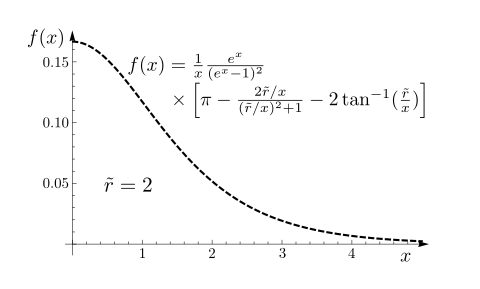
\includegraphics[width=0.49\textwidth]{behaviour_integrand.pdf}}
	\subfigure[Power dependence of the squared brackets multiplied by $\flatfrac{1}{x^{3}}$ in \eqref{eq:figure behaviour integrand}]{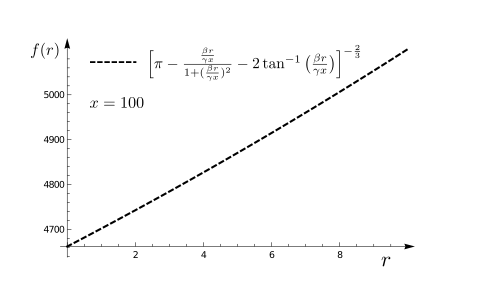
\includegraphics[width=0.49\textwidth]{dependence_integrand.pdf}}
	\caption{
On the left hand side, the behaviour of the integrand in equation \eqref{eq:figure behaviour integrand} is depicted for large und small values of $x$, where the factor $\tilde{r} = \flatfrac{r}{\gamma T}$ is set to 2.
The integrand function is convergent for large values due to the function decreases fast for large values of $x$.
For small values of $x$, the function takes a constanst value of $\flatfrac{4}{3\tilde{r}^{3}}$.
The integrand gets more divergent for small $x$, if the value $\tilde{r}$ decrease to zero.
The power dependence of the obtained momentum integral in \eqref{eq:figure behaviour integrand} is depicted on the right hand side, where $x=1000$.
Since the behaviour is linear, the investigated expression has the power of $-\flatfrac{3}{2}$.
	}
	\label{fig:behaviour integrand}
\end{figure}
%
A solution of the integral is evaluated determining the behaviour of the expression in squared brackets.
For large values of $x$, a linear $r$-dependence is given by the power of $-\flatfrac{3}{2}$.
This is depicted in the right hand side of figure \ref{fig:behaviour integrand}, where $x$ is set to $1000$.
An approximated expression is generated for the interand using the method of power counting.
The initial point of this approach is the momentum integral in euqtion \eqref{eq:starting expression}.
Numerator and differential yield in total the power of two, while the denominator generates the power of eight.
The integrand is a function proportional to $k^{-6}$ combing both powers.
The further approach is to investigate singularities of the integrand.
The limit $r \to 0$ or $\epsilon \to 0$ is seperately generated singularities in the function.
Both are considered with the power of three, since the power of them is half in comparison to the power of $k$ in equation \eqref{eq:starting expression}.
The integrand is therefore approximated by the following expression.
%
\begin{align}
	\Im{\mathcal{G}_{\dot{\mt{P}}\dot{\mt{P}}}^{\mt{ret}}(\vb{k}, z)} &\approx 
		-\frac{2 \vert \mt{J}_{\vb{G}} \vert^{2} \cdot G_{j}^{2}}{\gamma \pi^{2}} \cdot 
		\frac{\omega}{T}
		\int\limits_{0}^{\infty} \dd{x}
		\frac{x^{2} e^{x}}{(e^{x} - 1)^{2}}
		\frac{1}{(\tilde{r}^{2} + x^{2})^{\flatfrac{3}{2}}}
\end{align}
%
In figure \ref{fig:integrand exact vs approx}, the approximated expression is illustrated against the exact one.
The behaviour of both are nearly identical and the estimation is inspected to be valid.
The integrand decreases still fast to zero for $x \to \infty$, while the upper limit is set to some arbitrary cut-off $\Lambda$.
%
\begin{figure}[t]
	\centering
	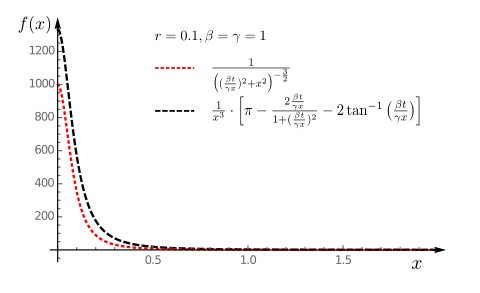
\includegraphics[width=0.6\textwidth]{original_vs_powercounting.pdf}
	\caption{
This figure shows the obtained expression of the momentum intgeral calculation (black curve, large strokes) in contrast to the obtained approximation using power counting technique (red curve, small strokes).
The used approximation is considered as good, since the characteristic of both curves is quite similar.
The value of $\tilde{r}$ is set to $0.1$.
	}
	\label{fig:integrand exact vs approx}
\end{figure}
%
The ratio of the exponential functions are then expanded for small values of $x$ up to the first non-vanishing order.
The remained integral is solved exactly while the solution of its is expanded for small $\flatfrac{\tilde{r}}{\Lambda}$.
%
\begin{align}
	\Im{\mathcal{G}_{\dot{\mt{P}}\dot{\mt{P}}}^{\mt{ret}}(\vb{k}, z)} &\approx 
		-\frac{2 \gamma \vert \mt{J}_{\vb{G}} \vert^{2} \cdot G_{j}^{2}}{\pi^{2} \Lambda} \cdot \frac{\omega T}{r^{2}}
\end{align}
%
To get the static electrical conductivity, this expression and the  approximated value of \eqref{eq:static susceptibility computed} is inserted into equation \eqref{eq:static conductivity formula}.
%
\begin{align}
	\sigma_{\mt{dc}}(T) = \frac{\mu\: m_{1}\: m_{2}\: \Lambda}{2\: \gamma\: \vert \mt{J}_{\vb{G}} \vert^{2}\: G_{j}^{2}} \cdot \frac{r^{2}}{T}
\end{align}
%
Beside the temperature itself, the only temperature dependent parameter is the control parameter $r$, which is proportional to the squard inverse correlation length, $r = \xi^{-2}$.
The correlation length is originated due to the fact that the system possesses a quantum phase transition and is temperature dependent is given by $\xi = T^{-1/z}$, as shown in chapter \ref{ch:spin fermion model}.
$z$ is a critical exponent and it is chosen in dependence of the temperature distance to the qantum critical point.
The corresponding temperature depencence of the control parameter is provided to $r = T^{2/z}$.
The resistance is determined by the inverse of the conductivity.
Considering only the temperature dependent parameters, the static resistance is given by
%
\begin{align}
	\rho_{\mt{dc}}(T) \sim T^{1-\flatfrac{4}{z}}.
	\label{eq:solution resistance}
\end{align}
%
Two possible choices are mentioned for the ciritcal exponent $z$.
In the vicinity of the quantum critical point at higher temperatures, $z$ is chosen to be one.
The $T$-dependence of the resistance is then given by $T^{-3}$.
In the limit $T \to 0$, this is highly divergent.
$z$ can be chosen to be 2 for lower temperatures.
Nevertheless, the $T$-dependence is evaluated to $T^{-1}$, which is still divergent in the limit $T \to 0$.

Our physial expectation is not confirmed with this divergent behaviour of the resistance.
Experiments of observed metals \cite{Loehneysen} are shown a linear temperature dependence of the resistance, $\rho(T) = \rho_{0} + A\: T$.
The behaviour of the resistance is therefore described incorrect using the obtained solution \eqref{eq:solution resistance}.
A possible origin of this disgrepancy between experiemnt and theory is maybe the diagrammatic pertubation theory.
In equation \eqref{eq:Green function}, the time evolution operator is expanded up to the first non-vanishing order.
This yields the free bubble diagram, while correction to the bubble are considered if the time evolution operator is expanded up to the next order.







%In Landau's Fermi liquid theory the resistance of a metal is given by $\rho(T) = \rho_{0} + A\: T^{2}$, where the residual resistance due to impurity scattering is represented by $\rho_{0}$.
%The $T^2$-dependence is originated by electron-electron scattering and umklapp-scattering \cite{Bader, Pal}


%In \cite{Loehneyesen} metals are investigated where a non-Fermi liquid behaviour 
%The consideration of umklapp scattering 

%Both results do not describe the physical results, presented in \cite{Loehneysen}.
%Here, 

%coincide 


















